% !TEX root = main.tex
\documentclass[10pt,twocolumn,letterpaper]{article}
\usepackage{cvpr}
% Shared packages for the CVPR-style review draft.
\usepackage{amsmath,amssymb,mathtools}
\usepackage{booktabs}
\usepackage{array}
\usepackage{multirow}
\usepackage{makecell}
\usepackage{graphicx}
\usepackage{xcolor}
\usepackage{tikz}
\usetikzlibrary{arrows.meta,positioning}
\usepackage{algorithm}
\usepackage{algpseudocode}
\usepackage{microtype}
\usepackage{xspace}

\newcommand{\method}{CRH-CFG\xspace}
\newcommand{\tbd}{\textcolor{red}{TBD}}
\newcommand{\R}{\mathbb{R}}
\newcommand{\E}{\mathbb{E}}
\newcommand{\hinge}[1]{\left[#1\right]_{+}}
\newcolumntype{P}[1]{>{\raggedright\arraybackslash}p{#1}}

% Include derivations and implementation details after the main paper.
\newif\ifincludesupplementary
\includesupplementarytrue


\definecolor{cvprblue}{rgb}{0.21,0.49,0.74}
\usepackage[pagebackref,breaklinks,colorlinks,allcolors=cvprblue]{hyperref}
\def\confName{CVPR}
\def\confYear{2026}

\title{Constraint-Aware Receding-Horizon Classifier-Free Guidance\\
for Attribute-Conditioned Flow Matching}
\author{Mu Chen}

\begin{document}
\maketitle

\begin{abstract}
Fixed-scale classifier-free guidance (CFG) is an open-loop policy for a
state- and time-varying generation process. We start from two structural facts.
First, once conditional and unconditional velocities are computed, all scalar
CFG actions lie on one affine line. Second, a straight Flow Matching path maps
each candidate velocity to an analytic clean-endpoint estimate. Together these
facts turn scale choice into a cheap finite control problem. We instantiate
this view as Constraint-Aware Receding-Horizon CFG (\method): a training-free
controller that repeatedly forecasts candidate endpoints and selects the
smallest temporally smooth action satisfying evaluator-based target and
protected-attribute constraints. The frozen generator and 50-step Heun solver
remain unchanged, and every method uses 100 guided-field evaluations (200 raw
U-Net forwards) per trajectory. On three CelebA attributes with 1,000 paired
seeds each, \method changes mean target success from 0.9840 to 0.9880 with
1.80\% mean wall-time overhead. This $+0.4$-point change is descriptive because
per-seed outcome transitions were not retained. Common-reference preservation
does not improve, and KID to the inherited full-marginal reference increases
for all targets but cannot identify conditional quality. The evidence therefore
supports low-overhead adaptive correction, not a joint improvement in
adherence, preservation, and quality.
\end{abstract}

\section{Introduction}

Flow Matching learns continuous transport by regressing a time-dependent
velocity field along a prescribed probability path \cite{lipman2023flow}.
Classifier-free guidance (CFG) sharpens conditional generation by affinely
combining conditional and unconditional predictions
\cite{ho2022classifierfree,zheng2023guided}. As with classifier-guided
diffusion \cite{dhariwal2021diffusion}, stronger guidance can improve semantic
alignment while sacrificing fidelity or diversity.

The usual fixed scale is structurally mismatched to the process it controls.
It applies one open-loop intervention to every initial noise and every stage,
even though a sample may already satisfy the condition or may become difficult
only later. Prior work on restricted intervals, condition annealing, early
suppression, and online feedback confirms that guidance demand is neither
uniform in time nor across samples
\cite{kynkaanniemi2024applying,sadat2024cads,fan2025cfgzerostar,papalampidi2025dynamic}.

Our starting point is the field structure itself. A conditional/unconditional
pair exposes only one scalar control direction, $g_s=v_c-v_u$, but it generates
every ordinary CFG candidate by affine recombination. For a straight path,
each candidate also yields an analytic prediction of its clean endpoint. Thus,
one expensive field pair can support many cheap, evaluator-scored actions. The
same equations expose the limitation: no selector can reach a desired effect
outside that one-dimensional action set.

\method turns this geometry into feedback. At selected states, it predicts a
finite bank of endpoints, filters candidates using target and protected-
attribute constraints, and chooses the least intervention with a temporal
smoothness penalty. An early reliability gate and a finite fallback make the
policy operational, while holding the selected scale across each Heun pair
keeps generator work exactly matched.

Our contributions are threefold: (1) a first-principles control view linking
the CFG affine line to straight-path endpoint prediction; (2) a vectorized,
training-free controller with explicit target, preservation, and minimum-
intervention terms; and (3) a paired, test-isolated evaluation that reports
both the small adherence point estimate and the observed evidence boundary,
rather than treating proxy feasibility as a quality guarantee.

\section{Related Work}

\paragraph{Flow Matching and classifier-free guidance.}
Flow Matching trains continuous normalizing flows by vector-field regression
along prescribed probability paths \cite{lipman2023flow}. Guided Flows
transfers classifier and classifier-free guidance to flow-based generation
\cite{zheng2023guided}. Standard CFG uses affine extrapolation of conditional
and unconditional predictions \cite{ho2022classifierfree}. \method retains
this frozen field and changes only the scalar selection policy.

\paragraph{When and how much to guide.}
Limited-interval guidance \cite{kynkaanniemi2024applying}, CFG-Zero*
\cite{fan2025cfgzerostar}, and condition annealing \cite{sadat2024cads}
modify when or how strongly a condition acts; rescaling is also coupled to the
noise schedule \cite{lin2023common}. Online feedback selects per-step scales
with auxiliary evaluators \cite{papalampidi2025dynamic}. \method is closest
to the latter, but its action set is exactly the ordinary CFG affine line, its
look-ahead comes from an analytic flow endpoint, and its selector explicitly
penalizes intervention while monitoring non-target attributes.

\paragraph{Guidance geometry and cost.}
Strong extrapolation can leave learned trajectories. CFG++ uses a
manifold-motivated correction \cite{chung2024cfgpp}, Rectified-CFG++ adapts
this view to flow models \cite{saini2025rectifiedcfgpp}, and manifold
projection directly targets Flow Matching scale sensitivity
\cite{cai2026improving}. Other work changes training to remove the two-branch
inference cost \cite{tang2025diffusion}. We make no manifold guarantee and do
not retrain: the original scalar direction is preserved, so reachability is
one-dimensional and evaluator overhead is separated from generator NFE.

\section{From Field Structure to Feedback}
\label{sec:problem}

\paragraph{Straight-path endpoint geometry.}
Let $s\in[0,1]$ increase from Gaussian noise $x_1$ to clean data $x_0$ along
the straight path
\begin{equation}
    x_s=(1-s)x_1+s x_0,\qquad
    \hat{x}_0(v)=x_s+(1-s)v.
    \label{eq:path}
\end{equation}
For the ideal bridge, $v=x_0-x_1$ makes the second relation exact. For a
learned field it is an analytic endpoint prediction, not a guarantee. The
paper/native clock conversion and derivation are given in
Appendix~\ref{app:derivation}.

\paragraph{One affine control axis.}
For condition $c$ and null condition $\varnothing$, define
$v_c=v_\theta(x_s,s,c)$, $v_u=v_\theta(x_s,s,\varnothing)$, and
$g_s=v_c-v_u$. Ordinary CFG satisfies
\begin{equation}
    v_w=v_u+w(v_c-v_u)=v_c+(w-1)g_s.
    \label{eq:cfg}
\end{equation}
With $a_s=w_s-1$, the sampler is control-affine,
\begin{equation}
    \frac{dY_s}{ds}=v_c(Y_s,s)+g_s(Y_s)a_s,
    \label{eq:control-affine}
\end{equation}
and Eq.~\eqref{eq:path} maps its complete action line to
\begin{equation}
    \hat{x}_0(w)=\hat{x}_0(1)+(1-s)(w-1)g_s.
    \label{eq:endpoint-locus}
\end{equation}
Thus, one conditional/unconditional pair defines every scalar action and its
predicted endpoint; it also fixes the local reachability boundary.

\paragraph{Least intervention under constraints.}
Because $w=1$ is the ordinary conditional field, we prefer actions near one
and near the previous decision, subject to a target margin and a protected-
attribute budget. Re-observing the state after integration and solving this
finite problem again yields receding-horizon feedback without multi-step
generator rollouts.

\section{Method: Constraint-Aware Receding-Horizon CFG}
\label{sec:method}

\begin{figure*}[t]
\centering
\resizebox{\textwidth}{!}{%
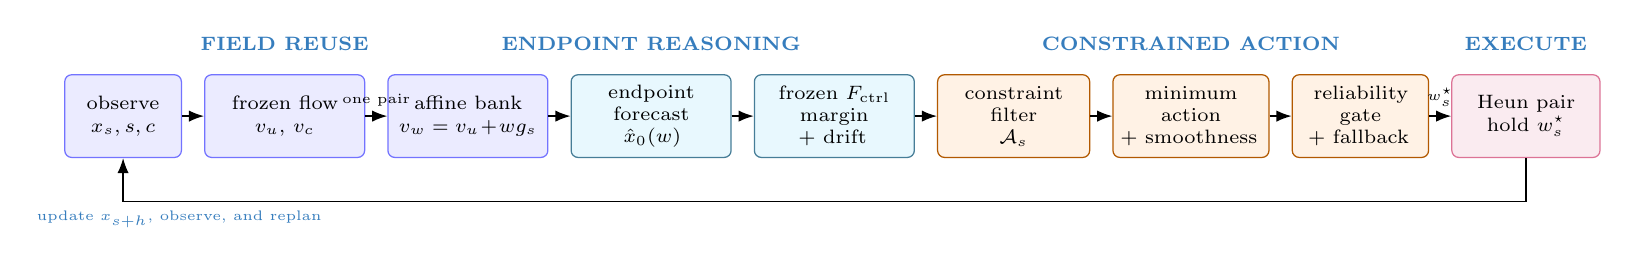
\begin{tikzpicture}[
    font=\scriptsize,
    >=Latex,
    box/.style={draw, rounded corners=2.5pt, align=center, minimum height=1.05cm,
                inner xsep=4pt, line width=0.45pt},
    field/.style={box, fill=blue!8, draw=blue!55},
    reason/.style={box, fill=cyan!9, draw=cyan!55!black},
    control/.style={box, fill=orange!10, draw=orange!70!black},
    execute/.style={box, fill=purple!8, draw=purple!55},
    flow/.style={->, line width=0.55pt},
    meta/.style={font=\scriptsize\bfseries, text=cvprblue, align=center}
]
\node[field, text width=1.20cm] (state) {observe\\$x_s,s,c$};
\node[field, text width=1.75cm, right=0.28cm of state] (unet)
    {frozen flow\\$v_u,\,v_c$};
\node[field, text width=1.75cm, right=0.28cm of unet] (bank)
    {affine bank\\$v_w=v_u+w g_s$};
\node[reason, text width=1.75cm, right=0.28cm of bank] (endpoint)
    {endpoint forecast\\$\hat x_0(w)$};
\node[reason, text width=1.75cm, right=0.28cm of endpoint] (eval)
    {frozen $F_{\rm ctrl}$\\margin + drift};
\node[control, text width=1.65cm, right=0.28cm of eval] (filter)
    {constraint filter\\$\mathcal A_s$};
\node[control, text width=1.70cm, right=0.28cm of filter] (select)
    {minimum action\\+ smoothness};
\node[control, text width=1.45cm, right=0.28cm of select] (gate)
    {reliability gate\\+ fallback};
\node[execute, text width=1.60cm, right=0.28cm of gate] (heun)
    {Heun pair\\hold $w_s^\star$};
\draw[flow] (state) -- (unet);
\draw[flow] (unet) -- node[above, font=\tiny] {one pair} (bank);
\draw[flow] (bank) -- (endpoint);
\draw[flow] (endpoint) -- (eval);
\draw[flow] (eval) -- (filter);
\draw[flow] (filter) -- (select);
\draw[flow] (select) -- (gate);
\draw[flow] (gate) -- node[above, font=\tiny] {$w_s^\star$} (heun);
\draw[flow] (heun.south) -- ++(0,-0.55) -| node[pos=0.48, below,
    font=\tiny, text=cvprblue] {update $x_{s+h}$, observe, and replan}
    (state.south);
\node[meta, above=0.18cm of unet] {FIELD REUSE};
\node[meta, above=0.18cm of endpoint] {ENDPOINT REASONING};
\node[meta, above=0.18cm of select] {CONSTRAINED ACTION};
\node[meta, above=0.18cm of heun] {EXECUTE};
\end{tikzpicture}%
}
\caption{\method follows the derivation from left to right: reuse one frozen
field pair, forecast the affine candidate endpoints, select a feasible
minimum intervention, execute it, and re-observe. Candidate expansion and
endpoint scoring add no generator calls. $F_{\rm eval}$ is outside this loop
and is used only for final measurement.}
\label{fig:method-overview}
\end{figure*}

\subsection{Candidate Endpoint Bank}

At each decision, the candidate set is
$\mathcal{W}=\{0.5,1.0,1.5,2.0,3.0,4.0\}$. Conditional and unconditional
fields are evaluated once, after which candidate velocities and endpoints are
constructed in parallel:
\begin{align}
    v_{w_m} &= v_u+w_m(v_c-v_u),\quad w_m\in\mathcal{W},
    \label{eq:candidates}\\
    \hat{x}_0(w_m) &= x_s+(1-s)v_{w_m}.
    \label{eq:candidate-endpoints}
\end{align}
The frozen controller evaluator scores all endpoints in one batch. For target
$a$, desired sign $y_a$, and protected set $P_a$, we use
\begin{align}
M_a(w,s)&=y_aF_{\mathrm{ctrl},a}(\hat{x}_0(w)),
    \label{eq:target-margin}\\
D_{\mathrm{nt}}(w,s)&=\frac{1}{|P_a|}\sum_{j\in P_a}
\left|F_{\mathrm{ctrl},j}(\hat{x}_0(w))-F_{\mathrm{ctrl},j}(\hat{x}_0(1))\right|.
    \label{eq:protected-drift}
\end{align}
The second quantity is a local attribute-logit proxy relative to $w=1$, not
an identity or perceptual-similarity guarantee.

\subsection{Constraint-Aware Minimum Intervention}

The feasible action set is
\begin{equation}
    \mathcal{A}_s=\left\{w\in\mathcal{W}:M_a(w,s)\geq m(s),\quad
    D_{\mathrm{nt}}(w,s)\leq\epsilon(s)\right\}.
    \label{eq:feasible-set}
\end{equation}
If $\mathcal{A}_s$ is nonempty, the controller selects
\begin{equation}
    w_s^\star=\arg\min_{w\in\mathcal{A}_s}
    \rho(w-1)^2+\eta(w-w_{\mathrm{prev}})^2.
    \label{eq:feasible-objective}
\end{equation}
This is the central design rule: satisfy the online proxies, then use the
least change from ordinary conditional generation and the previous action.
If the feasible set is empty, a finite hinge-penalty objective returns the
least-violating candidate and records the violated constraints. Full schedules,
normalization, and the fallback are in Appendix~\ref{app:controller-details}.

\subsection{Receding-Horizon Execution}

Validation selected the default scale $w=2$ for $s<\tau_{\mathrm{on}}=0.1$,
where predicted endpoints are least reliable. Thereafter, the controller is
evaluated every five Heun macro-steps and the previous scale is held between
decisions. The chosen $w_s^\star$ is held across the Heun predictor--corrector
pair; only then is $x_{s+h}$ observed and the problem replanned. Static CFG and
\method therefore both execute 100 guided fields, or 200 conditional/
unconditional U-Net forwards, per trajectory. \method adds ten batched
evaluator decisions, but no generator trajectories. The exact Heun update,
algorithm, and complexity are in Appendix~\ref{app:controller-details}.

\section{Experimental Protocol}
\label{sec:experiments}

\paragraph{Frozen generator and data.}
We freeze the 18.5M-parameter, $64\times64$ attribute-conditioned U-Net and its
50,000-iteration EMA checkpoint. The inherited CelebA subset contains 63,715
images \cite{liu2015celeba}; a deterministic split isolates controller
training, validation, and final test data. We evaluate positive Smiling, Bangs,
and Blond Hair requests. Architecture and split counts are in
Appendix~\ref{app:experimental-details}.

\paragraph{Methods and paired protocol.}
The five methods are static $w=2$, validation-selected interval CFG,
target-only feedback, target-plus-preservation feedback, and full \method.
Every comparison shares checkpoint, EMA weights, conditions, initial noises,
and the 50-step Heun solver. Each target uses the same 1,000 seeds across
methods; ablations use the first 256. Controller schedules and penalties are
frozen on validation data and listed in Appendix~\ref{app:experimental-details}.

\paragraph{Evaluators and metrics.}
$F_{\mathrm{ctrl}}$ selects actions; a separately fine-tuned
$F_{\mathrm{eval}}$ measures final target success and protected-logit drift.
Both use ImageNet-pretrained ResNet-18 features \cite{he2016resnet}, so
independent heads and fine-tuning do not eliminate correlated representation
error. CelebA annotations are also imperfect \cite{wu2023celeba}. A common,
same-seed $w=1$ reference makes preservation comparisons meaningful. KID
\cite{binkowski2018mmd} uses the inherited full CelebA marginal; it measures
closeness to that marginal, not conditional-target quality. Evaluator accuracy,
KID sampling details, and metric definitions are in the appendix.

\section{Results}
\label{sec:results}

\subsection{Main Comparison}

\begin{table*}[t]
\caption{Main results on 1,000 paired seeds per target. All methods use the
same frozen generator and 50-step Heun solver. Drift and flip are relative to
the paired static $w=2$ result; $\mathrm{KID}_{\mathrm{marg}}$ is mean $\pm$
subset standard deviation against the inherited full-marginal reference. All
rows use 100 guided-field evaluations.}
\label{tab:main-results}
\centering
\scriptsize
\setlength{\tabcolsep}{3.15pt}
\begin{tabular}{llrrrrrrr}
\toprule
Target & Method & Succ. $\uparrow$ & $\Delta$ pp & Drift $\downarrow$ &
Flip $\downarrow$ & $\mathrm{KID}_{\mathrm{marg}}\downarrow$ & $\bar w$ & $\Delta$ time \\
\midrule
\multirow{5}{*}{Smiling}
& Static $w=2$ & .985 & +0.0 & .0000 & .0000 & $.01223\!\pm\!.00063$ & 2.0000 & +0.00\% \\
& Interval & .979 & -0.6 & .1169 & .0037 & $.01173\!\pm\!.00060$ & -- & -0.50\% \\
& Target only & .860 & -12.5 & 1.5417 & .0498 & $.00904\!\pm\!.00050$ & 1.0739 & +2.30\% \\
& Target + pres. & .860 & -12.5 & 1.5417 & .0498 & $.00904\!\pm\!.00050$ & 1.0739 & +2.54\% \\
& \textbf{Full \method} & \textbf{.987} & \textbf{+0.2} & .0025 & .0003 & $.01223\!\pm\!.00063$ & 2.0067 & +2.70\% \\
\midrule
\multirow{5}{*}{Bangs}
& Static $w=2$ & .980 & +0.0 & .0000 & .0000 & $.04110\!\pm\!.00162$ & 2.0000 & +0.00\% \\
& Interval & .972 & -0.8 & .2707 & .0093 & $.04087\!\pm\!.00161$ & -- & -0.07\% \\
& Target only & .888 & -9.2 & 3.1288 & .1258 & $.02379\!\pm\!.00126$ & 1.1952 & +1.61\% \\
& Target + pres. & .888 & -9.2 & 3.1288 & .1258 & $.02379\!\pm\!.00126$ & 1.1952 & +1.97\% \\
& \textbf{Full \method} & \textbf{.984} & \textbf{+0.4} & .0476 & .0018 & $.04123\!\pm\!.00162$ & 2.0480 & +1.58\% \\
\midrule
\multirow{5}{*}{Blond}
& Static $w=2$ & .987 & +0.0 & .0000 & .0000 & $.06872\!\pm\!.00225$ & 2.0000 & +0.00\% \\
& Interval & .986 & -0.1 & .3156 & .0095 & $.06711\!\pm\!.00221$ & -- & +0.07\% \\
& Target only & .972 & -1.5 & 1.7170 & .0555 & $.05884\!\pm\!.00206$ & 1.2571 & +1.47\% \\
& Target + pres. & .972 & -1.5 & 1.7170 & .0555 & $.05884\!\pm\!.00206$ & 1.2571 & +1.29\% \\
& \textbf{Full \method} & \textbf{.993} & \textbf{+0.6} & .2858 & .0070 & $.07083\!\pm\!.00229$ & 2.1689 & +1.12\% \\
\bottomrule
\end{tabular}
\end{table*}

Table~\ref{tab:main-results} shows a consistent but small positive adherence
point estimate. Full \method changes the unweighted mean success from 0.9840
to 0.9880, or $+0.4$ percentage points. Target-wise counts change from
985/1,000 to 987/1,000 for Smiling, 980 to 984 for Bangs, and 987 to 993 for
Blond Hair. Because the artifact retains aggregate counts but not per-seed
success transitions, McNemar or paired-bootstrap uncertainty cannot be
reconstructed. These values are descriptive and do not establish a
statistically reliable or large practical improvement.

Closeness to the inherited full-marginal reference moves in the opposite
direction. Relative to static $w=2$, full \method changes
$\mathrm{KID}_{\mathrm{marg}}$ by $+0.00001$, $+0.00013$, and $+0.00211$ for
Smiling, Bangs, and Blond Hair. The first two changes are small relative to the
reported subset standard deviations, which are not confidence intervals for
method differences. Since the reference mixes positive and negative examples,
these increases do not identify a decline in conditional quality. The main
hypothesis is nevertheless unsupported because common-reference preservation
does not improve; conditional quality remains unresolved under this KID
reference.

The frozen-feature diversity results reinforce the same trade-off
(Table~\ref{tab:diversity}). Target-only control is more diverse for every
attribute because it selects substantially lower scales. Full \method remains
close to static CFG for Smiling and Bangs and is less diverse for Blond Hair
(.2579 to .2515, a 2.46\% relative decrease). Its unweighted mean changes from
.3532 to .3507. This feature-space proxy has no confidence interval, so it is
descriptive rather than inferential. No method is uniformly better on observed
success, marginal-reference KID, protected drift, diversity, and wall time.

\begin{figure*}[t]
\centering
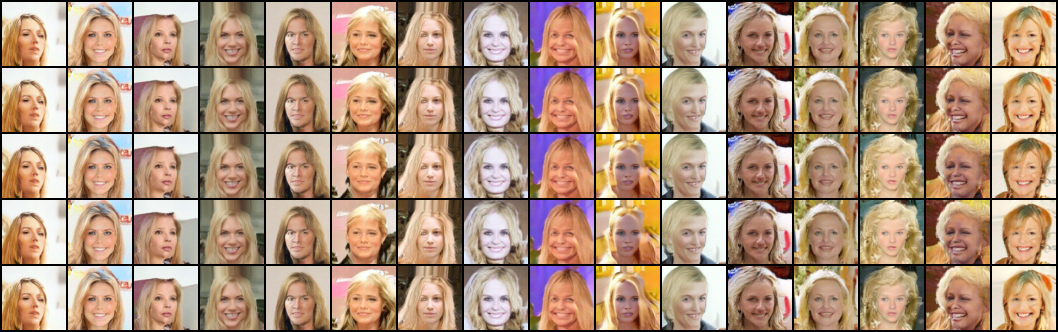
\includegraphics[width=\textwidth]{../figures/blond_hair_paired_methods.png}
\caption{Paired Blond Hair generations for the first 16 frozen seeds. Rows are
static $w=2$, interval CFG, target-only control, target-plus-preservation, and
full \method. The two reduced controllers are visually and numerically
identical, while the full controller remains close to static CFG. This grid is
seed-ordered and not selected by image quality.}
\label{fig:paired-blond}
\end{figure*}

\begin{table}[t]
\caption{Mean cosine distance between paired random samples in frozen
$F_{\mathrm{eval}}$ backbone features. Higher denotes greater feature
diversity. Target-only and target-plus-preservation are identical.}
\label{tab:diversity}
\centering
\small
\setlength{\tabcolsep}{3.3pt}
\begin{tabular}{lrrrr}
\toprule
Target & Static & Interval & Target & Full \\
\midrule
Smiling & .3729 & .3750 & .4383 & .3724 \\
Bangs & .4290 & .4344 & .4858 & .4281 \\
Blond & .2579 & .2637 & .2885 & .2515 \\
\bottomrule
\end{tabular}
\end{table}

\subsection{A Common Preservation Reference}

Baseline-relative drift in Table~\ref{tab:main-results} cannot establish that
static CFG preserves the ordinary conditional solution because its own drift is
zero by construction. Table~\ref{tab:common-reference} instead compares all
methods with paired $w=1$ trajectories and averages only after retaining
target-wise records.

\begin{table}[t]
\caption{Unweighted mean preservation diagnostic against common, same-seed
$w=1$ outputs. Lower drift and flip imply closer protected attributes, but can
coincide with lower target success.}
\label{tab:common-reference}
\centering
\small
\setlength{\tabcolsep}{3.8pt}
\begin{tabular}{lrrr}
\toprule
Method & Success $\uparrow$ & Drift $\downarrow$ & Flip $\downarrow$ \\
\midrule
Static $w=2$ & .9840 & 2.7770 & .0963 \\
Interval & .9790 & 2.7596 & .0973 \\
Target / target+pres. & .9067 & 1.1067 & .0318 \\
Full \method & .9880 & 2.8433 & .0980 \\
\bottomrule
\end{tabular}
\end{table}

Full \method is slightly farther from $w=1$ than static CFG on both common
reference metrics. Target-only and target-plus-preservation stay substantially
closer, but lose 7.73 mean success points. The selected controller therefore
exposes a target--preservation trade-off rather than a preservation win.

\subsection{Component and Hyperparameter Evidence}

\begin{table}[t]
\caption{Component ablation on 256 seeds per target, reported as unweighted
target means. KID uses the reduced 100-image/50-subset full-marginal-reference
protocol and is not comparable with Table~\ref{tab:main-results}.}
\label{tab:components}
\centering
\scriptsize
\setlength{\tabcolsep}{2.6pt}
\begin{tabular}{@{}lrrrr@{}}
\toprule
Variant & Succ. & Drift & Flip & KID \\
\midrule
Static $w=2$ & .9857 & .0000 & .0000 & .04152 \\
Target feedback & .8503 & 2.9184 & .1104 & .02595 \\
Target + pres. & .8503 & 2.9184 & .1104 & .02595 \\
Target + min. int. & .9063 & 2.0954 & .0749 & .03070 \\
Target + pres. + min. & .9063 & 2.0954 & .0749 & .03070 \\
Full package & .9883 & .0833 & .0036 & .04224 \\
Full, no gate & .9154 & 1.8887 & .0677 & .03480 \\
Full, fixed threshold & .9870 & .5143 & .0169 & .04476 \\
\bottomrule
\end{tabular}
\end{table}

Table~\ref{tab:components} yields three conclusions. First, feedback without
the full regularized package moves toward $w=1$ and sacrifices adherence.
Second, adding the preservation term changes no reported value, both with and
without minimum intervention. The selected budget is therefore non-binding in
these variants. Third, removing the early reliability gate drops mean success
from 0.9883 to 0.9154; this comparison validates the full package, but does not
isolate smoothness from every simultaneous design change.

The preregistered $w_{\max}$ sweep is consistent with limited extra control
authority. Increasing $w_{\max}$ from 2 to 3 changes success from 0.9857 to
0.9883 while increasing drift from 0.0004 to 0.0775 and reduced KID from
0.04152 to 0.04215. Raising it to 4 leaves success at 0.9883. Sweeping the
endpoint parameter $\epsilon(1)\in\{0.25,0.5,1.0\}$, corresponding to actual
last-decision budgets $\epsilon(.9)\in\{.425,.650,1.100\}$, produces identical
aggregate values. This further confirms that the preservation constraint does
not determine the chosen actions.

\subsection{Controller Dynamics and Failures}

\begin{figure}[t]
\centering
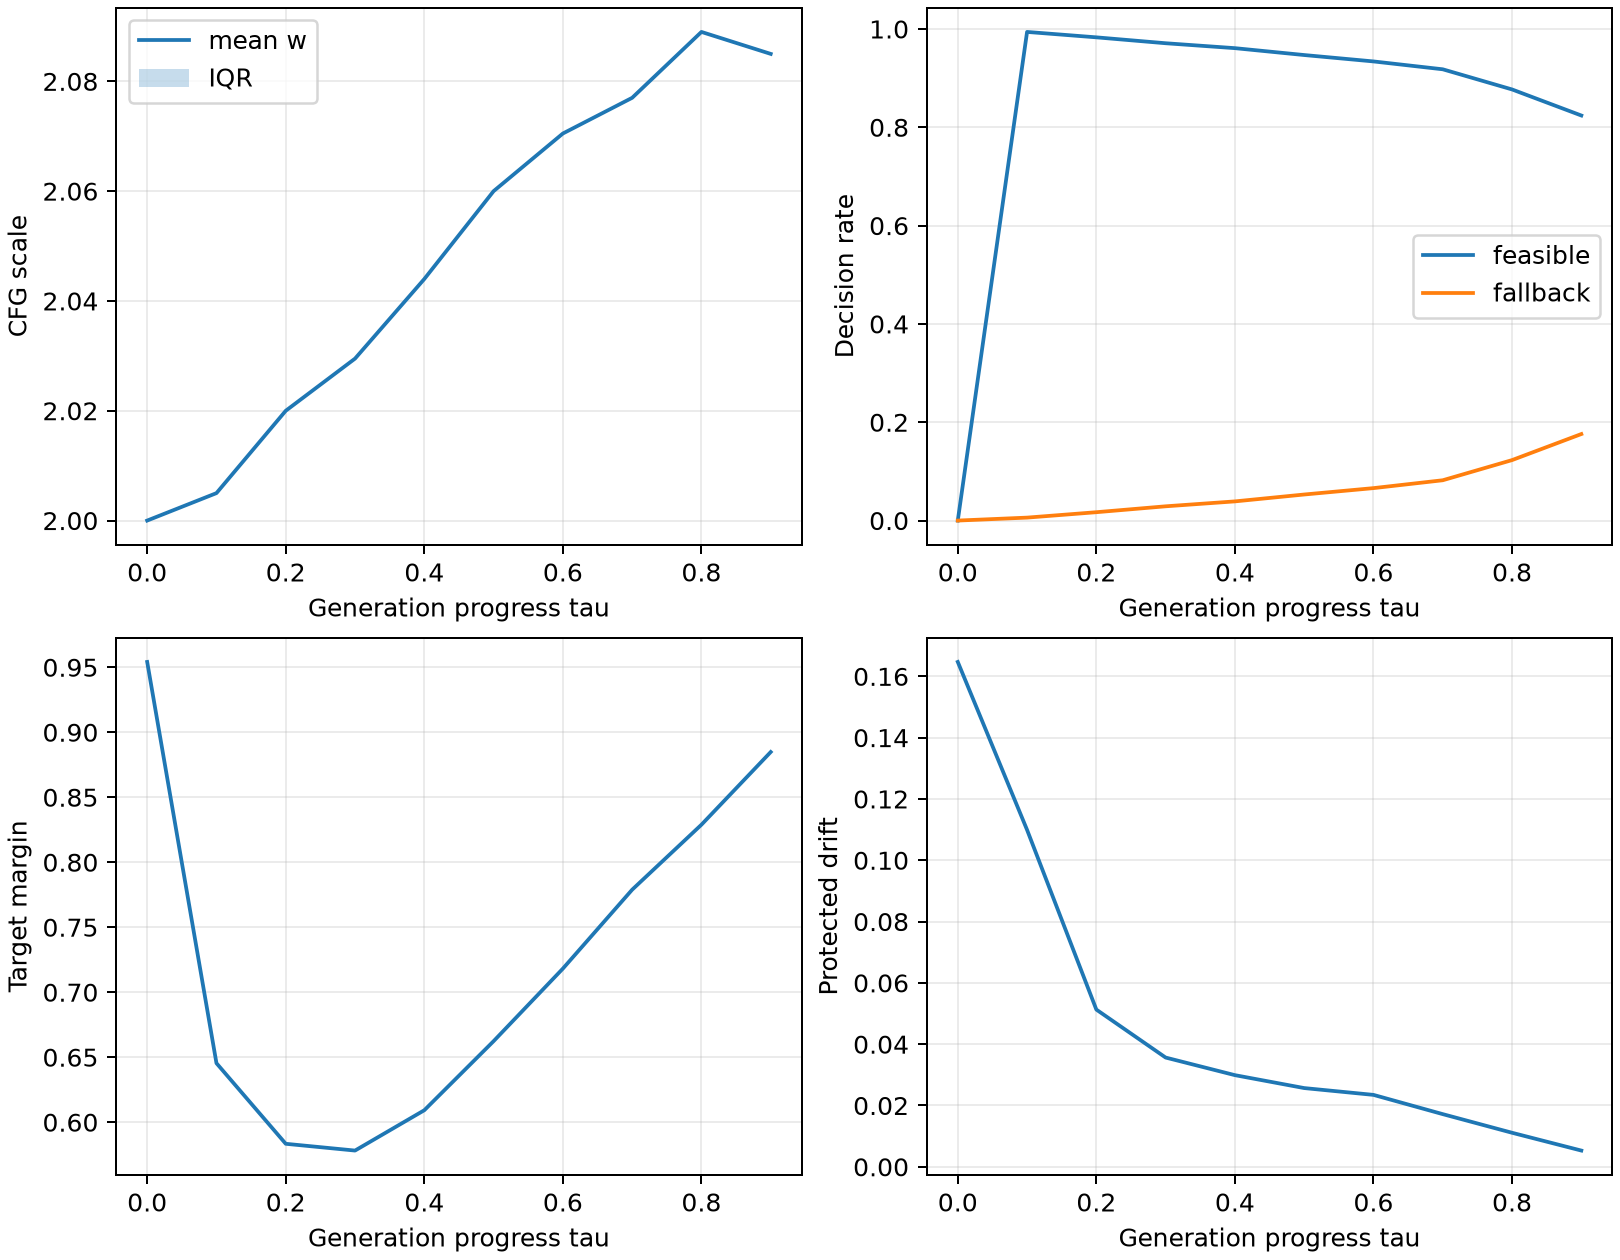
\includegraphics[width=\linewidth]{../figures/bangs_present_schedule.png}
\caption{Full-controller dynamics for Bangs over 1,000 trajectories. The
median and interquartile scale remain 2, while the fallback rate rises late in
sampling. This is the target with the highest final fallback rate.}
\label{fig:bangs-schedule}
\end{figure}

The controller is adaptive for a minority of difficult samples, but the
population policy remains close to static CFG. At $s=0.9$, mean scales are
2.0170, 2.0850, and 2.1855 for Smiling, Bangs, and Blond Hair; the median and
interquartile scale remain 2 at every saved decision. Final fallback rates are
0.057, 0.176, and 0.016, with feasible rates 0.943, 0.824, and 0.984. Bangs is
thus the least frequently feasible target, whereas Blond Hair receives the
strongest late intervention and exhibits both the largest positive adherence
point estimate and the largest increase in marginal-reference KID.

\begin{table}[t]
\caption{Controller state at the final saved decision $s=0.9$. Although mean
scale differs by target, all scale medians and interquartile ranges equal 2.}
\label{tab:schedule-summary}
\centering
\small
\begin{tabular}{lrrr}
\toprule
Target & Mean $w$ & Feasible & Fallback \\
\midrule
Smiling & 2.0170 & .943 & .057 \\
Bangs & 2.0850 & .824 & .176 \\
Blond Hair & 2.1855 & .984 & .016 \\
\bottomrule
\end{tabular}
\end{table}

\begin{figure*}[t]
\centering
\begin{minipage}[t]{0.325\textwidth}
\centering
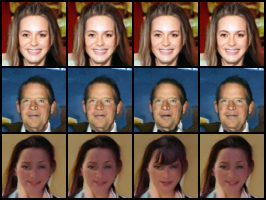
\includegraphics[width=\linewidth]{../figures/smiling_present_selected_cases.png}\\[-2pt]
{\small (a) Smiling}
\end{minipage}\hfill
\begin{minipage}[t]{0.325\textwidth}
\centering
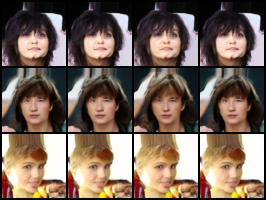
\includegraphics[width=\linewidth]{../figures/bangs_present_selected_cases.png}\\[-2pt]
{\small (b) Bangs}
\end{minipage}\hfill
\begin{minipage}[t]{0.325\textwidth}
\centering
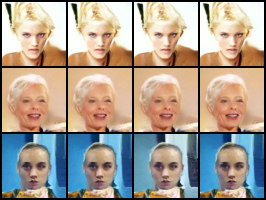
\includegraphics[width=\linewidth]{../figures/blond_hair_selected_cases.png}\\[-2pt]
{\small (c) Blond Hair}
\end{minipage}
\caption{Rule-selected paired cases. Within each panel, columns are static
$w=2$, interval CFG, target-only control, and full \method; rows are the
maximum-margin success, the case closest to the independent evaluator boundary,
and the minimum-margin failure. Selection uses frozen statistics rather than
visual preference.}
\label{fig:qualitative}
\end{figure*}

The rule-selected failures clarify the method boundary. For Smiling seed
410577, the static and full signed margins are $-10.291$ and $-10.139$, and the
controller falls back at 30\% of decisions despite reaching $w=3$. For Bangs
seed 410550, fallback reaches 80\%, the maximum selected scale remains 2, and
the final margin worsens from $-6.201$ to $-7.777$. For Blond Hair seed 410327,
the controller reaches $w=4$ and improves the margin from $-7.205$ to $-5.250$
without crossing the decision boundary. These cases show insufficient scalar
control authority and imperfect transfer from predicted endpoints scored by
$F_{\mathrm{ctrl}}$ to final outcomes scored by $F_{\mathrm{eval}}$.

\subsection{Cost}

Full \method matches generator work exactly and increases mean wall time by
1.80\% across targets. Its candidate tensors and evaluator batches raise peak
memory from 644,830,208 to 673,739,776 bytes, an increase of 27.6 MiB. The
measured HW4 study, including calibration, main experiments, ablations, and
analysis, consumed 3.824 L40S GPU-hours. The retained HW3 timestamps imply an
additional 2.6875 GPU-hours for generator training, explicitly an estimate
rather than a billing record.

The artifact audit checks exact seed coverage, sample and trajectory counts,
finite metric values, frozen checkpoint hashes, the deterministic split hash,
and agreement between aggregate CSV rows and paper tables. Nineteen automated
tests cover time conversion, endpoint prediction, candidate vectorization,
fallback behavior, Heun scale holding, paired-seed reproducibility, split
isolation, checkpoint freezing, and matched generator NFE. These checks do not
validate the semantic proxy, but they separate implementation failures from
the empirical limitations observed above.

\section{Discussion and Limitations}
\label{sec:discussion}

\paragraph{What is supported.}
The full policy is a conservative correction around $w=2$, not a broadly new
sampler. Smoothness and the early gate prevent the collapse toward $w=1$ seen
in reduced variants, giving a small positive adherence point estimate at
matched generator work. The non-binding preservation term explains why the
full policy inherits static CFG's preservation behavior; the study therefore
supports low-overhead adaptive correction, not the intended joint benefit.

\paragraph{Structural and proxy limits.}
Equation~\eqref{eq:control-affine} gives only one local control direction. If
every point on the affine line violates a constraint, replanning cannot create
new authority. Endpoint estimates are also least reliable near noise, and both
online constraints depend on $F_{\mathrm{ctrl}}$. The separate evaluator
reduces direct reuse but shares architecture and pretrained features. Useful
extensions are uncertainty-aware evaluator ensembles and independently
validated control directions; both require new matched-compute baselines.

\paragraph{Evidence limits.}
Across 3,000 trajectories, static CFG records 2,952 successes and \method
records 2,964. Because per-seed outcome transitions were not retained, this net
difference cannot support a paired significance test. KID subset deviations
are not confidence intervals, and the marginal reference cannot identify
conditional quality. The results describe one checkpoint, dataset, resolution,
solver, and three positive requests rather than generalization across models
or data regimes.

\paragraph{Scope and responsible use.}
Protected-logit drift measures selected attributes, not identity, perceptual
similarity, fairness, or consent. CelebA labels are noisy and correlated
\cite{wu2023celeba}; appearance labels can encode social assumptions. The
method should not be interpreted as reliable real-person editing or
sensitive-attribute control.

\section{Conclusion}

Starting from the CFG affine control axis and the straight-path endpoint map,
we derived \method as finite, minimum-intervention feedback for a frozen flow.
It preserves solver and generator evaluation counts and adds 1.80\% mean wall
time. Across three paired 1,000-sample targets, mean success changes by a
descriptive $+0.4$ points, while common-reference preservation does not improve
and conditional quality remains unresolved by marginal-reference KID. The
method is therefore a low-overhead adaptive correction with an explicit
one-dimensional reachability boundary, not evidence for a universal joint win.

{
    \small
    \bibliographystyle{ieeenat_fullname}
    \bibliography{main}
}

\ifincludesupplementary
\clearpage
\appendix

\section{Time Conventions and Endpoint Derivation}
\label{app:derivation}

The paper-time convention runs from data to noise,
\begin{equation}
    x_t=(1-t)x_0+t x_1,\qquad t=0\text{ data},\quad t=1\text{ noise}.
    \label{eq:path-paper-appendix}
\end{equation}
Its ideal bridge velocity is $u_t=x_1-x_0$, so
\begin{equation}
    x_t-tu_t=(1-t)x_0+t x_1-t(x_1-x_0)=x_0.
    \label{eq:data-pred-paper}
\end{equation}
The implementation uses the native generation clock $s=1-t$ and the reverse
velocity $v_s=-u_t=x_0-x_1$. Substitution gives
\begin{equation}
    \hat{x}_0=x_s+(1-s)v_s=x_t-tu_t.
    \label{eq:data-pred-native}
\end{equation}
This equality is exact for the ideal straight bridge. With a learned velocity,
the same expression is a one-step endpoint forecast.

For CFG, $v_w-v_1=(w-1)(v_c-v_u)=(w-1)g_s$. The native endpoint map then
implies
\begin{align}
\hat{x}_0(w)-\hat{x}_0(1)
&=(1-s)(v_w-v_1)\\
&=(1-s)(w-1)g_s,
\end{align}
which yields Eq.~\eqref{eq:endpoint-locus}. This derivation explains both the
computational reuse and the one-dimensional reachability limit; it does not
assert that evaluator scores vary monotonically with $w$.

\section{Controller and Solver Details}
\label{app:controller-details}

\paragraph{Schedules and normalization.}
Each controller-evaluator margin is divided by its validation-only standard
deviation, preserving its zero decision boundary. The target threshold and
protected budget are
\begin{align}
m(s)&=m_{\mathrm{early}}+
  (m_{\mathrm{late}}-m_{\mathrm{early}})s^\gamma,
  \label{eq:threshold}\\
\epsilon(s)&=\epsilon_{\mathrm{early}}+
  (\epsilon_{\mathrm{late}}-\epsilon_{\mathrm{early}})s.
  \label{eq:budget}
\end{align}
Decisions occur at $s\in\{0,.1,\ldots,.9\}$. Therefore, the ``late'' values
parameterize the schedule endpoint at $s=1$ rather than an observed decision.
For the frozen configuration, the final decision uses $m(.9)=.567$ and
$\epsilon(.9)=.650$.

\paragraph{Fallback.}
When $\mathcal{A}_s$ is empty, \method minimizes the finite objective
\begin{align}
J_s(w)=&\ \alpha\hinge{m(s)-M_a(w,s)}
+\lambda\hinge{D_{\mathrm{nt}}(w,s)-\epsilon(s)}\nonumber\\
&+\rho(w-1)^2+\eta(w-w_{\mathrm{prev}})^2,
\qquad w\in\mathcal{W}.
\label{eq:fallback}
\end{align}
Because $\mathcal{W}$ is finite and nonempty, the fallback always returns a
candidate. The implementation separately logs target, preservation, and joint
violations.

\paragraph{Heun integration.}
With $h=1/50$, predictor and corrector share the selected action:
\begin{align}
\tilde{x}_{s+h}&=x_s+h\,v_{w_s^\star}(x_s,s),\\
x_{s+h}&=x_s+\frac{h}{2}\left[v_{w_s^\star}(x_s,s)+
v_{w_s^\star}(\tilde{x}_{s+h},s+h)\right].
\label{eq:heun}
\end{align}
Holding $w_s^\star$ avoids changing the numerical protocol inside a macro-step.

\begin{algorithm}[h]
\caption{\method{} with Heun Protocol B}
\label{alg:crh}
\begin{algorithmic}[1]
\Require Frozen $\theta$, state $x$, condition $c$, candidate set $\mathcal W$,
evaluator $F_{\mathrm{ctrl}}$
\State $w_{\mathrm{prev}}\gets1$
\For{$k=0,\ldots,49$}
    \State Compute $(v_u,v_c)$ once at the current state
    \If{$k$ is a controller decision}
        \State Construct and score all endpoints by
        Eqs.~\eqref{eq:candidates}--\eqref{eq:candidate-endpoints}
        \State Select $w^\star$ by Eq.~\eqref{eq:feasible-objective}
        or Eq.~\eqref{eq:fallback}
    \Else
        \State $w^\star\gets w_{\mathrm{prev}}$
    \EndIf
    \State Apply one Heun step, holding $w^\star$ for the corrector
    \State $w_{\mathrm{prev}}\gets w^\star$
\EndFor
\State \Return $x$
\end{algorithmic}
\end{algorithm}

For batch size $B$ and $M=|\mathcal W|$, candidate endpoints form an
$M\times B\times C\times H\times W$ tensor, clipped to $[-1,1]$ and evaluated
in one batch. Construction costs $O(MBCHW)$ tensor work plus one controller
evaluator pass over $MB$ images per decision. It does not launch an additional
generator trajectory.

\section{Experimental Details}
\label{app:experimental-details}

The frozen conditional U-Net has base width 64, channel multipliers
$[1,2,2,4]$, two residual blocks per level, attention at $16\times16$, four
attention heads, and 18,535,619 parameters. The seed-42 data permutation fixes
50,972 training, 6,371 validation, and 6,372 final-test images. Main experiments
use seeds 410000--410999 for each target and method; ablations use the first 256.

\begin{table}[ht]
\caption{Validation-frozen controller configuration.}
\label{tab:controller-config}
\centering
\small
\setlength{\tabcolsep}{4pt}
\begin{tabular}{@{}ll@{}}
\toprule
Component & Value \\
\midrule
Candidate scales & $\{0.5,1,1.5,2,3,4\}$ \\
Target schedule & $m(0)=-.5$, $m(1)=.75$, $\gamma=1.5$ \\
Drift budget & $\epsilon(0)=2.0$, $\epsilon(1)=.5$, linear \\
Penalties & $(\alpha,\lambda,\rho,\eta)=(1,1,.05,.20)$ \\
Reliability gate & $s<0.1$, default $w=2$ \\
Decision period & Every 5 of 50 macro-steps \\
\bottomrule
\end{tabular}
\end{table}

$F_{\mathrm{eval}}$ is independently fine-tuned from the same fixed ImageNet
initialization as $F_{\mathrm{ctrl}}$, using new heads and training seed 31,415.
It is trained on inherited training indices, selected on validation, and opens
final-test labels only in the final phase.

\begin{table}[ht]
\caption{Separately fine-tuned $F_{\mathrm{eval}}$ performance on real final-
test images. These labels are not used by the controller.}
\label{tab:evaluator}
\centering
\small
\begin{tabular}{lrr}
\toprule
Attribute & Accuracy & AUROC \\
\midrule
Smiling & .8991 & .9626 \\
Bangs & .9510 & .9771 \\
Black Hair & .8788 & .9335 \\
Blond Hair & .9317 & .9684 \\
Brown Hair & .7960 & .8786 \\
\bottomrule
\end{tabular}
\end{table}

Main KID uses 1,000 generated images, the complete 63,715-image inherited real
marginal, subset size 1,000, and 100 fixed subsets. The reference positive
prevalence is 44.42\% for Smiling, 15.87\% for Bangs, and 11.13\% for Blond
Hair. Ablations use subset size 100 and 50 subsets; the two protocols are not
pooled.

\section{Metric Definitions}

Let $N$ paired samples be indexed by $i$, target sign be $y_a$, and final
independent-evaluator margin be $z_{i,a}$. Target success is
\begin{equation}
    \mathrm{Success}_a=\frac{1}{N}\sum_{i=1}^{N}
    \mathbf{1}\!\left[y_a z_{i,a}\geq0\right].
\end{equation}
For reference method $r$ and protected set $P_a$, paired logit drift is
\begin{equation}
    \mathrm{Drift}_{a,r}=\frac{1}{N|P_a|}
    \sum_{i=1}^{N}\sum_{j\in P_a}
    \left|z_{i,j}^{\mathrm{method}}-z_{i,j}^{r}\right|.
\end{equation}
Protected flip rate counts changes in margin sign. The common-reference
diagnostic uses paired ordinary conditional $w=1$ trajectories for $r$.

\section{Reproducibility Ledger}

\begin{table}[ht]
\caption{Frozen experiment ledger.}
\centering
\footnotesize
\begin{tabular}{@{}p{0.28\linewidth}p{0.66\linewidth}@{}}
\toprule
Item & Frozen value \\
\midrule
Generator & 18,535,619-parameter conditional U-Net; EMA checkpoint; no HW4
updates \\
Integrator & 50 Heun macro-steps; selected scale held per predictor--corrector
pair \\
Main seeds & 410000--410999 for each target and method \\
Ablation seeds & First 256 main seeds for each target \\
Controller & Ten decisions per trajectory; gate for $s<0.1$ \\
Main KID & 1,000 generated; 63,715 real; subset 1,000; 100 subsets \\
Reduced KID & 256 generated; subset 100; 50 subsets \\
Tests & 19 implementation and protocol tests passed \\
\bottomrule
\end{tabular}
\end{table}

\section{Failure Records}

\begin{table}[ht]
\caption{Rule-selected failures with independent-evaluator signed margins.}
\centering
\scriptsize
\setlength{\tabcolsep}{2.7pt}
\begin{tabular}{@{}lrrrrr@{}}
\toprule
Target / seed & Static & Full & Max $w$ & Fallback & Drift \\
\midrule
Smiling / 410577 & -10.291 & -10.139 & 3 & .30 & .184 \\
Bangs / 410550 & -6.201 & -7.777 & 2 & .80 & 1.197 \\
Blond / 410327 & -7.205 & -5.250 & 4 & .10 & .126 \\
\bottomrule
\end{tabular}
\end{table}

For Smiling, local feedback does not reverse failure. For Bangs, all late
candidates miss the target threshold. For Blond Hair, stronger intervention
improves the margin but does not reach success.
\fi

\end{document}
